\subsection{Bathymetry}
\label{sec: bathy}

	Survey data collected on 1 October 2015 was considered for this analysis. These data were measured via the CRAB and Trimble Real Time Kinematic (RTK) GPS system. Elevation data from six cross-sections, perpendicular to the shoreline, spaced over a 100-meter portion of the beach were combined to create the 2D surface shown in Figure \ref{2D Bath}. 
	
	 	\begin{figure}[H]
	 	\centering
	 	%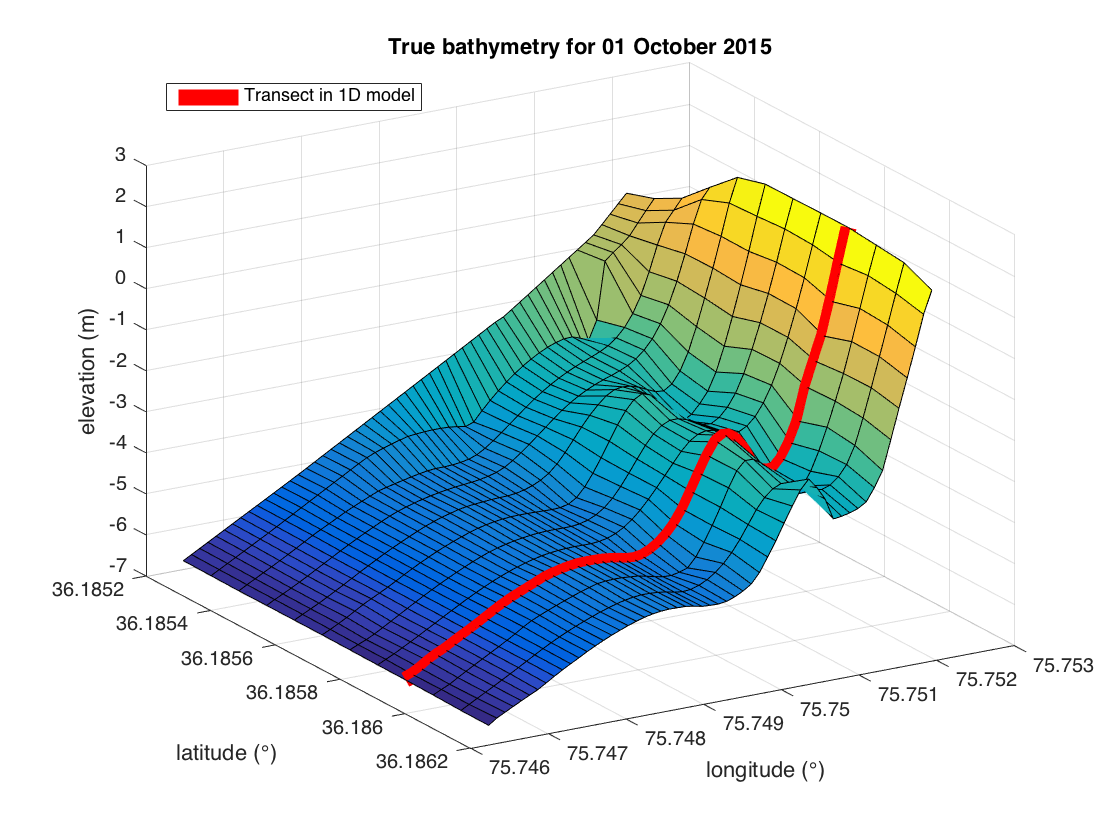
\includegraphics[width=0.6\linewidth]{img/trueBath2D.png}
	 	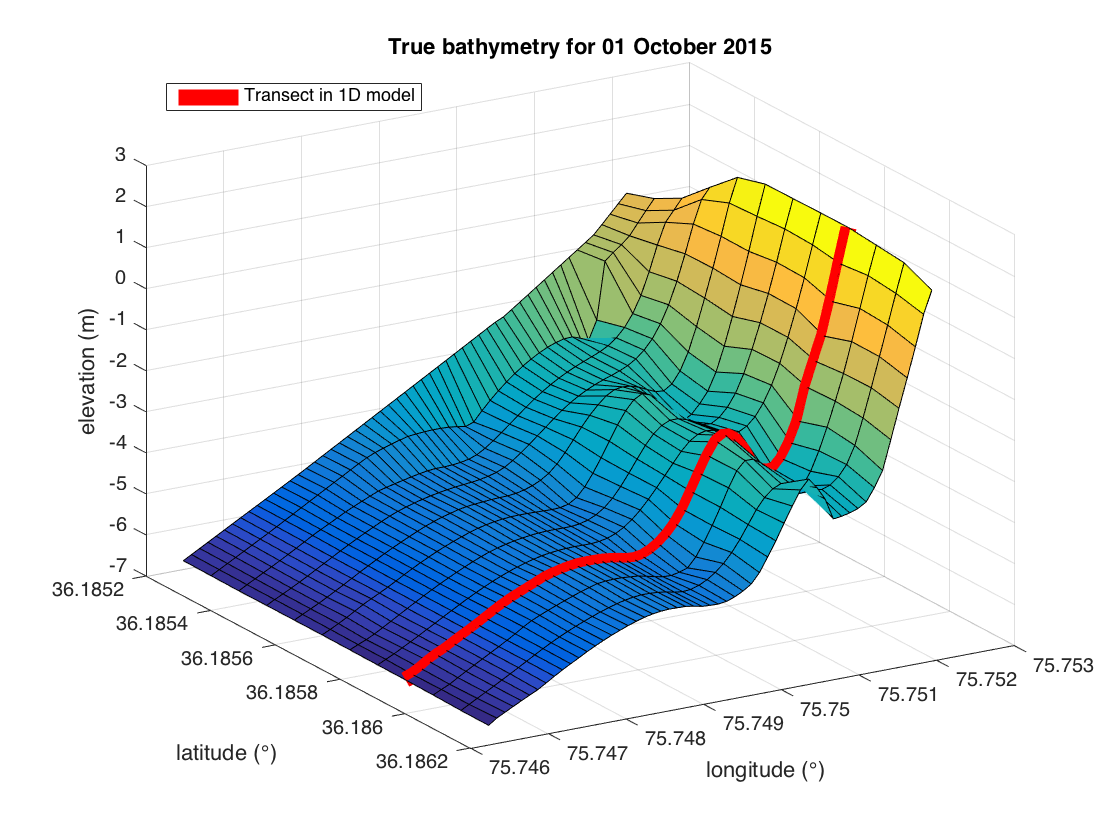
\includegraphics[width=0.5\linewidth]{img/trueBath2D.png}
	 	\caption{Measured and gridded 2D bathymetry in the survey area on 1 October 2015. The red line shows the transect considered in the 1D problem.}
	 	\label{2D Bath}
	 	\end{figure}
	
	For the 1D problem, a single slice of the 2D bathymetry was used as model input, identified by the red line in Figure \ref{2D Bath}. In a cartesian coordinate system, this line (a.k.a. `transect') is located at \textit{y} = 950 meters. 
		
		\begin{figure}[H]
		\centering
		%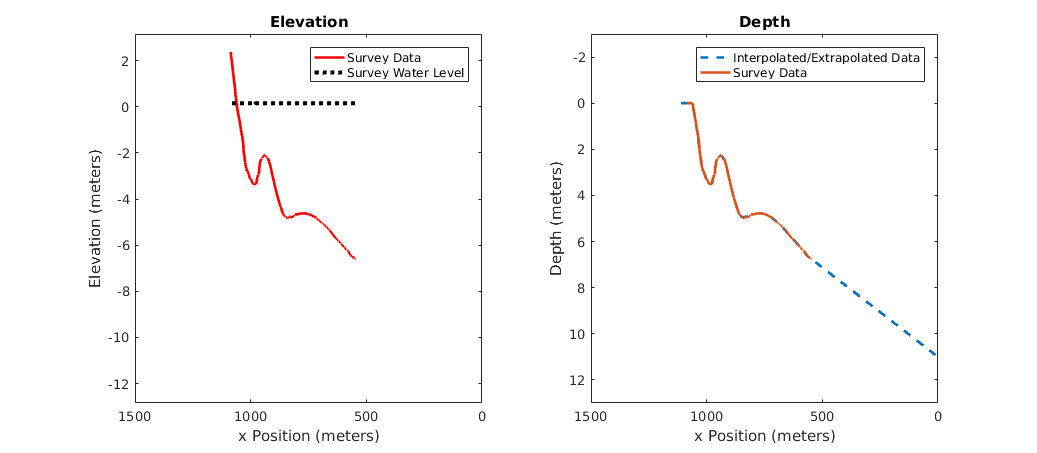
\includegraphics[width = 1.0\linewidth]{img/trueBath1D.png}
		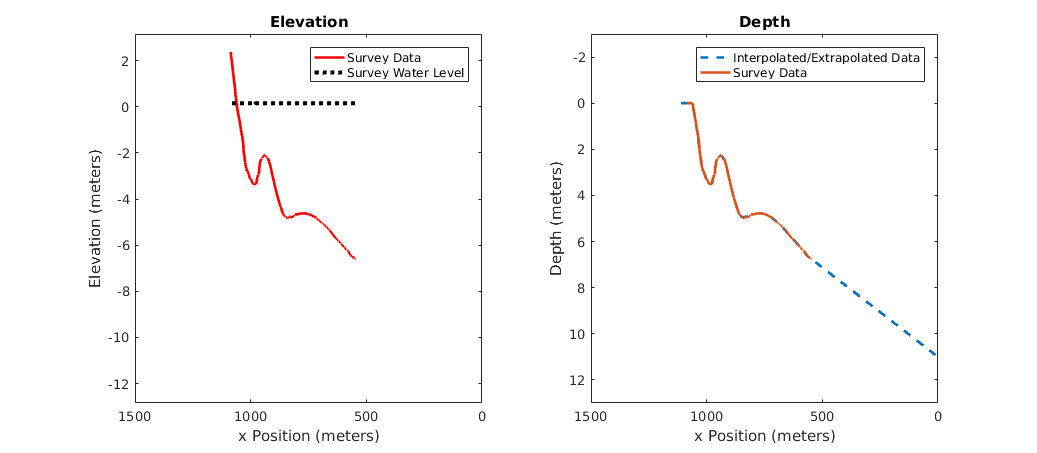
\includegraphics[width = 0.65\linewidth]{img/trueBath1D.png}
		\caption{1D Bathymetry - elevation data (left) and depth data (right).}
		\label{1D Bath}
		\end{figure}
		
	Survey data provided sea floor elevation referenced to the North American Vertical Datum of 1988 (NAVD88) (Figure \ref{1D Bath}, \textit{left}). To provide proper input data for the 1D model, elevation was transformed to depth data (Figure \ref{1D Bath}, \textit{right}). Once transformed, depth was discretized by interpolating between measured data points via Matlab's built-in pchip method. Pchip was chosen for the interpolation due to its shape-preserving nature so as to not introduce non-physical oscillations. Between the boundary condition and the nearest measured depth point, linear interpolation was used to fill in missing data.